\documentclass[runningheads]{llncs}

% ---------------------------------------------------------------------------
% Packages
% ---------------------------------------------------------------------------
\usepackage[T1]{fontenc}
\usepackage[utf8]{inputenc}
\usepackage{graphicx}
\usepackage{amsmath,amssymb}
\usepackage{booktabs}
\usepackage{array}
\usepackage{multirow}
\usepackage{xcolor}
\usepackage{tikz}
\usetikzlibrary{arrows.meta,positioning,fit,backgrounds,calc}
\usepackage[hidelinks]{hyperref}

\graphicspath{{figures/}}

% Compact column type
\newcolumntype{C}[1]{>{\centering\arraybackslash}p{#1}}

\begin{document}

% ---------------------------------------------------------------------------
% Title
% ---------------------------------------------------------------------------
\title{A Gated Multimodal Architecture with Stochastic Weight Averaging for
Directional Trading Decisions over Heterogeneous Financial Assets}

\titlerunning{Gated Multimodal Fusion with SWA for Trading Decisions}

\author{First Author\inst{1} \and
Second Author\inst{2} \and
Third Author\inst{1}}

\authorrunning{F. Author et al.}

\institute{Institution One, City, Country\\
\email{\{author1,author3\}@institution.edu}
\and
Institution Two, City, Country\\
\email{author2@institution.edu}}

\maketitle

% ---------------------------------------------------------------------------
% Abstract
% ---------------------------------------------------------------------------
\begin{abstract}
We address the engineering of a computational architecture able to ingest and
synchronize heterogeneous information sources for daily directional trading
decisions: continuous price series, high-frequency unstructured text processed
through a financial language model, and discrete low-frequency corporate
filings. The central difficulty is not modelling each modality in isolation but
fusing them coherently under severe asymmetries in frequency, dimensionality and
availability. We propose a four-branch network that couples a patch-based
temporal encoder, an attention pooling module over FinBERT news embeddings, a
filing projection with temporal decay, and a per-day scalar encoder, integrated
through a gated fusion layer that masks branches whose evidence is absent or
inapplicable to the instrument. The architecture is validated on the FinMMEval
Task~3 corpus (twelve assets spanning equities and cryptocurrencies). We
contribute three engineering decisions: a per-asset volatility-adaptive
labelling scheme, the decoupling of model optimization from decision-threshold
optimization to curb overfitting on a temporally small validation set, and the
use of Stochastic Weight Averaging (SWA). On the held-out test partition the
validation-selected model attains a cumulative return of \textbf{23.3\%}, an
annualized Sharpe ratio of \textbf{4.21}, and a maximum drawdown of
\textbf{4.45\%}. We deliberately frame this as a validation-selected operating
point rather than an expected value: across five seeds the test Sharpe varies
widely (standard deviation $\approx 1.9$), a direct consequence of the short
evaluation window. We further document two negative results---SWA does not raise
the across-seed mean, and prediction ensembles degraded out-of-sample
performance---and argue that in this low-data regime the binding constraint is
the experimental protocol rather than model capacity. All metrics are reported
with explicit statistical caveats.

\keywords{Multimodal fusion \and Deep learning \and Financial NLP \and FinBERT
\and Gated attention \and Stochastic Weight Averaging \and FinMMEval.}
\end{abstract}

% ---------------------------------------------------------------------------
\section{Introduction}
% ---------------------------------------------------------------------------
Predicting the short-term direction of financial assets is a canonical testbed
for multimodal learning. Market behaviour emerges from the interaction of price
dynamics, the flow of textual information, and discrete corporate events, each
differing in sampling frequency, granularity and semantics. The engineering
challenge is to design an architecture that \emph{synchronizes and weights}
these signals without allowing high-cardinality modalities to dominate sparse but
informative ones, and without forcing the model to integrate evidence that does
not exist for a given instrument on a given day.

This work centres on the \emph{architectural engineering} of multimodal fusion;
the financial task serves as a controlled validation case rather than as the
objective in itself. The same design concerns recur in any domain where
continuous sensor streams, free text and discrete events must be combined.

Our contributions are: (i) a four-branch architecture with \emph{gated fusion
and availability masking}, where each modality can be differentiably silenced
when its evidence is null or inapplicable; (ii) a \emph{per-asset
volatility-adaptive labelling} scheme that balances the class distribution
across instruments with disparate volatility profiles; (iii) a training protocol
that \emph{separates model optimization from decision optimization}, fixing the
activation threshold during training and tuning it only once at evaluation; (iv)
the integration of \emph{Stochastic Weight Averaging} (SWA)~\cite{izmailov2018}
as an implicit regularizer, with an ablation quantifying its effect; and (v) a
transparent \emph{negative result} on ensembling, which degraded out-of-sample
performance in our low-data regime.

% ---------------------------------------------------------------------------
\section{Related Work}
% ---------------------------------------------------------------------------
Deep learning for financial forecasting has been surveyed
extensively~\cite{sezer2020}. News-driven prediction was popularized by
event-embedding models~\cite{ding2015} and attention-based frameworks that
weight news by relevance~\cite{hu2018}. The introduction of domain-adapted
language models, notably FinBERT~\cite{yang2020,araci2019}, enabled robust
sentiment and representation extraction from financial text. For the price
stream, transformer encoders~\cite{vaswani2017} have been adapted to time series;
PatchTST~\cite{nie2023} showed that segmenting a series into subseries-level
patches yields strong, parameter-efficient forecasters.

Multimodal fusion has a well-established taxonomy~\cite{baltrusaitis2019}. Gated
multimodal units~\cite{arevalo2017} learn per-modality importance weights, a
mechanism we extend with an explicit availability mask so that inapplicable
modalities (e.g.\ filings for cryptocurrencies) are excluded by construction.
On the optimization side, SWA~\cite{izmailov2018} averages weights along the
training trajectory to reach flatter optima that generalize better, and
decoupled weight decay~\cite{loshchilov2019} stabilizes adaptive optimizers.
For labelling, the difficulty of defining directional targets under
non-stationary volatility is discussed in the financial machine-learning
literature~\cite{lopezdeprado2018}; we adopt a per-asset percentile dead-zone
instead of a global static threshold.

% ---------------------------------------------------------------------------
\section{Problem Formulation and Data}
% ---------------------------------------------------------------------------
\subsection{Multimodal formulation}
For an asset at day $t$ we observe
$\mathcal{X}_t = \{\mathbf{S}_t,\ \mathcal{N}_t,\ \mathcal{E}_t\}$, where
$\mathbf{S}_t \in \mathbb{R}^{L \times d_s}$ is a window of $L$ days of scalar
technical features, $\mathcal{N}_t=\{n_t^{(1)},\dots,n_t^{(k_t)}\}$ is a
variable-size set of news headlines, and $\mathcal{E}_t$ encodes corporate
filings (10-K, 10-Q). The goal is a function
$f_\theta:\mathcal{X}_t \mapsto y_t \in \{\textsc{sell},\textsc{hold},\textsc{buy}\}$
producing one daily recommendation per asset.

\subsection{Corpus}
The corpus is provided by the \emph{FinMMEval Task~3} framework and is built from
the publicly released \texttt{daily\_news} collection accessed from the Hugging
Face Hub (\texttt{TheFinAI/daily\_news}). It comprises twelve assets---ten US equities (AAPL, ADBE, AMZN,
BMRN, GOOGL, META, MRNA, MSFT, NVDA, TSLA) and two cryptocurrencies (BTC,
ETH)---over the period 2025-08-01 to 2026-04-25. Each daily record contains the
closing price, a momentum tag, the set of news for the day, and optional
filings. Table~\ref{tab:dataset} summarizes the dataset after preprocessing.

For equities, weekend and holiday records (no trading) are removed and their
news are carried forward to the next trading day with an exponential temporal
decay $w=\exp(-\lambda\,\Delta_{\text{days}})$, $\lambda=0.18$, so that Friday
news reaching Monday retain weight $\approx 0.70$. Cryptocurrencies trade seven
days a week and require no consolidation. Temporal splits are performed per asset
(65\%/15\%/20\%) and concatenated, preserving chronological order and preventing
look-ahead leakage.

\begin{table}[t]
\centering
\caption{Dataset summary after weekend consolidation and tensorization.}
\label{tab:dataset}
\begin{tabular}{ll}
\toprule
Property & Value \\
\midrule
Assets & 12 (10 equities, 2 crypto) \\
Date range & 2025-08-01 to 2026-04-25 \\
Raw daily records & 2{,}446 \\
Trading days per equity / crypto & 191 / 268 \\
Tensorized samples (train/val/test) & 1{,}588 / 360 / 496 \\
Unique trading dates (val / test) & 40 / 53 \\
Train class balance (S/H/B) & 524 / 529 / 535 \\
Scalar features selected & 19 (of 69 candidates) \\
Sequence length $L$ & 30 days \\
Max news per day & 8 \\
News / filings coverage & all days / equities only \\
\bottomrule
\end{tabular}
\end{table}

% ---------------------------------------------------------------------------
\section{Methodology}
% ---------------------------------------------------------------------------
\subsection{Feature engineering and dynamic labelling}
A single feature-engineering module is shared between offline training and the
serving runtime, guaranteeing reproducibility. From roughly sixty candidate
indicators (returns at multiple horizons, realized volatilities, RSI, MACD,
Bollinger position, trend slopes, calendar dummies, news counts, filing-decay
features and cross-asset proxies) we select $19$ features through the combination
of Spearman correlation, mutual information, LightGBM~\cite{ke2017} gain under a
purged walk-forward cross-validation with a five-day embargo, and a variance
inflation factor filter to remove collinear variables.

\paragraph{Target construction.}
Let $r_{t,a}=(p_{t+1,a}-p_{t,a})/p_{t,a}$ be the one-day-ahead realized return.
A per-asset \emph{dead-zone} threshold $\tau_a$ is estimated as the
$q$-th percentile of $|r|$ over an initial in-sample window $W_a$ of each asset
(the first $70\%$ of its series):
\begin{equation}
\tau_a = \mathrm{P}_{q}\big(\{|r_{s,a}| : s \in W_a\}\big),
\qquad q = 33,
\end{equation}
and the categorical label is
\begin{equation}
y_{t,a}=
\begin{cases}
\textsc{buy}, & r_{t,a} > +\tau_a,\\
\textsc{sell}, & r_{t,a} < -\tau_a,\\
\textsc{hold}, & |r_{t,a}| \le \tau_a.
\end{cases}
\end{equation}
A static global threshold under-represents the active class for low-volatility
instruments and over-represents noise for volatile ones. The per-asset
percentile produces thresholds ranging from $0.18\%$ (MSFT) to $0.86\%$ (ETH),
which track each instrument's volatility and keep the three classes
approximately balanced (Table~\ref{tab:dataset}). An auxiliary regression target,
the return normalized by a 20-day rolling realized volatility (lagged one day to
avoid leakage), supervises a secondary head.

\paragraph{On the estimation window and look-ahead.}
The window $W_a$ (first $70\%$) is slightly wider than the $65\%$ training split,
so it overlaps the first few validation days; it never reaches the test
partition. This is deliberate and has no measurable effect on the reported
results, for two reasons. First, $\tau_a$ is a single per-asset \emph{magnitude}
derived from $|r|$ (no directional or future information) and, empirically,
recomputing it on the strict $65\%$ training split leaves \emph{all} $360$
validation labels unchanged and alters only $2$ of $496$ test labels ($0.4\%$);
model selection, which is performed on validation, is therefore invariant.
Second, the headline financial metrics (CR, SR, MD, DV, AV) are computed from
realized returns and the model's discrete signals and are \emph{independent of}
$\tau_a$, which enters only the auxiliary classification metrics (accuracy and
macro-F1). The reported test performance is thus free of look-ahead.

\subsection{Architecture}
\label{sec:methodology-arch}
The model (Fig.~\ref{fig:arch}) has four modality branches whose
$d$-dimensional outputs are integrated by a gated fusion layer. Identity
information---an 8-dimensional learned symbol embedding concatenated with an
asset-type flag---is appended before the output heads, so the network always
knows which instrument it is scoring.

\begin{figure}[t]
\centering
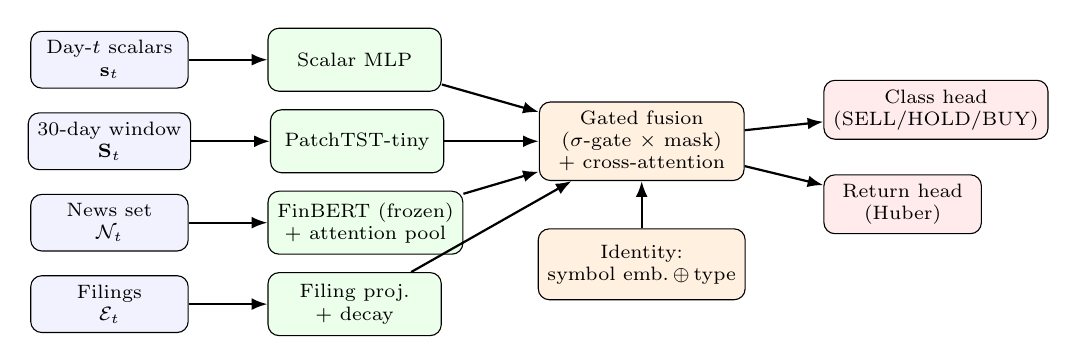
\begin{tikzpicture}[
  font=\scriptsize,
  box/.style={draw, rounded corners, align=center, minimum height=7mm, minimum width=20mm, fill=blue!5},
  enc/.style={draw, rounded corners, align=center, minimum height=8mm, minimum width=22mm, fill=green!8},
  fuse/.style={draw, rounded corners, align=center, minimum height=9mm, minimum width=26mm, fill=orange!12},
  head/.style={draw, rounded corners, align=center, minimum height=7mm, minimum width=20mm, fill=red!8},
  arr/.style={-{Latex[length=2mm]}, thick}
]
% inputs
\node[box] (s1) {Day-$t$ scalars\\$\mathbf{s}_t$};
\node[box, below=3mm of s1] (s2) {30-day window\\$\mathbf{S}_t$};
\node[box, below=3mm of s2] (s3) {News set\\$\mathcal{N}_t$};
\node[box, below=3mm of s3] (s4) {Filings\\$\mathcal{E}_t$};
% encoders
\node[enc, right=10mm of s1] (e1) {Scalar MLP};
\node[enc, right=10mm of s2] (e2) {PatchTST-tiny};
\node[enc, right=10mm of s3] (e3) {FinBERT (frozen)\\+ attention pool};
\node[enc, right=10mm of s4] (e4) {Filing proj.\\+ decay};
% fusion
\node[fuse, right=12mm of e2] (gate) {Gated fusion\\($\sigma$-gate $\times$ mask)\\+ cross-attention};
\node[fuse, below=6mm of gate] (id) {Identity:\\symbol emb.\,$\oplus$\,type};
% heads
\node[head, right=10mm of gate, yshift=4mm] (h1) {Class head\\(SELL/HOLD/BUY)};
\node[head, right=10mm of gate, yshift=-8mm] (h2) {Return head\\(Huber)};
% arrows
\foreach \a/\b in {s1/e1,s2/e2,s3/e3,s4/e4} \draw[arr] (\a) -- (\b);
\foreach \e in {e1,e2,e3,e4} \draw[arr] (\e) -- (gate);
\draw[arr] (gate) -- (h1);
\draw[arr] (gate) -- (h2);
\draw[arr] (id) -- (gate);
\end{tikzpicture}
\caption{Multimodal architecture. Four modality branches feed a gated fusion
layer with availability masking; learned identity features are appended before
the classification and regression heads. FinBERT is frozen; only $115$K
parameters are trained.}
\label{fig:arch}
\end{figure}

\paragraph{Branches.}
(1) A scalar MLP encodes the day-$t$ feature vector. (2) A compact
PatchTST~\cite{nie2023} encoder segments the 30-day window into non-overlapping
patches of length five and applies a two-layer transformer with mean pooling.
(3) News are embedded with a frozen FinBERT (\texttt{finbert-tone})~\cite{yang2020};
the day's headlines are aggregated by an attention pooling whose query is the
concatenation of the symbol embedding and the asset-type flag, with attention
logits additively biased by the temporal decay weight. (4) A filing projection
encodes the running filing embedding after applying a 45-day half-life decay.

\subsection{Gated fusion with availability masking}
Let $\mathbf{h}_m \in \mathbb{R}^{d}$ be the representation of branch $m$ and
$a_m\in\{0,1\}$ its availability indicator ($a_{\text{filing}}=0$ for crypto;
$a_{\text{news}}=0$ on days without news). A gate is computed from the
concatenation of all branches and modulated by availability:
\begin{equation}
g_m = \sigma\!\big(W_g\,[\mathbf{h}_1 \Vert \cdots \Vert \mathbf{h}_4]\big)_m \cdot a_m .
\end{equation}
Gated representations $g_m\mathbf{h}_m$ are refined by light cross-attention
across the four branches (treated as tokens) and pooled with weights
proportional to $g_m$. This design prevents the network from being forced to
integrate non-existent evidence.

\subsection{Loss, optimization and stabilization}
The objective is multi-task,
$\mathcal{L} = \alpha\,\mathcal{L}_{\text{CE}} + (1-\alpha)\,\mathcal{L}_{\text{Huber}}$,
with $\alpha=0.8$, class-balanced cross-entropy with label
smoothing~\cite{szegedy2016} of $0.10$, and a Huber loss on the
volatility-normalized return. We optimize with AdamW~\cite{loshchilov2019} under
a five-epoch warmup and cosine decay, with gradient clipping and three temporal
data augmentations (Gaussian feature noise, news dropout, window time-shift).

\paragraph{Decoupling decision from optimization.}
Converting class probabilities into a discrete action requires an activation
threshold $\theta$. Optimizing $\theta$ jointly with the weights---selecting,
each epoch, the value that maximizes a financial metric on validation---induces
overfitting when the validation set has \emph{few unique trading dates} (here,
40). The annualized Sharpe ratio over so few days has large sampling variance,
and a fine threshold sweep exploits accidents of the particular realization.
We therefore (i) hold $\theta=0.50$ \emph{fixed} during training and select the
model by a combined score $0.5\,\tanh(\mathrm{SR}/3)+0.5\,\mathrm{F1}$ that is
robust to the threshold, and (ii) tune $\theta$ \emph{once} on validation after
training, by grid search in $[0.34,0.70]$, transferring the chosen value to the
test set.

\paragraph{Stochastic Weight Averaging.}
SWA~\cite{izmailov2018} averages the weights visited in the final training phase,
$\bar{\theta}_{\text{SWA}}=\frac{1}{K}\sum_{k} \theta_k$, approximating the
centre of a flat region of the loss surface. Flat minima are less sensitive to
distribution shift between validation and test, which is the dominant failure
mode in this low-data regime. We start averaging at epoch~30 with a reduced
constant learning rate and recompute normalization statistics with one
post-training pass over the training set. The averaged checkpoint is evaluated
as an independent model.

% ---------------------------------------------------------------------------
\section{Experimental Setup}
% ---------------------------------------------------------------------------
Table~\ref{tab:hyper} lists the hyperparameters of the deployed configuration.
The model has $115{,}016$ trainable parameters (the frozen FinBERT encoder is
excluded). We report portfolio-level metrics computed on daily returns
aggregated across assets with equal weight over active (non-\textsc{hold})
positions, annualizing with a factor of $252$:
Cumulative Return (CR), annualized Sharpe Ratio (SR), Maximum Drawdown (MD),
Daily Volatility (DV) and Annualized Volatility (AV)~\cite{sharpe1994}. The
threshold selected on validation is transferred unchanged to the test set.

\begin{table}[t]
\centering
\caption{Hyperparameters of the deployed configuration.}
\label{tab:hyper}
\begin{tabular}{lll}
\toprule
Component & Hyperparameter & Value \\
\midrule
\multirow{4}{*}{Architecture}
 & Fusion dimension $d$ & 32 \\
 & PatchTST layers / patch length & 2 / 5 \\
 & Symbol embedding dim & 8 \\
 & Trainable parameters & 115{,}016 \\
\midrule
\multirow{6}{*}{Optimization}
 & Optimizer & AdamW \\
 & Learning rate & $1\times10^{-3}$ \\
 & Weight decay & $1\times10^{-2}$ \\
 & Batch size & 32 \\
 & Dropout & 0.35 \\
 & Max epochs / warmup / patience & 80 / 5 / 20 \\
\midrule
\multirow{3}{*}{Loss}
 & $\alpha$ (CE weight) & 0.80 \\
 & Label smoothing & 0.10 \\
 & Class weights & balanced \\
\midrule
\multirow{3}{*}{Augmentation}
 & Gaussian noise $\sigma$ & 0.03 \\
 & News dropout prob.\ & 0.30 \\
 & Time shift & $\pm 2$ \\
\midrule
\multirow{2}{*}{SWA}
 & Start epoch & 30 \\
 & SWA learning rate & $5\%$ of base \\
\bottomrule
\end{tabular}
\end{table}

% ---------------------------------------------------------------------------
\section{Results}
% ---------------------------------------------------------------------------
\subsection{Main results}
We compare four checkpoints, all sharing the architecture of
Section~\ref{sec:methodology-arch} and the same corpus and splits. The
\emph{prior baseline} is an earlier checkpoint of the identical architecture
($d{=}32$, two PatchTST layers, dropout $0.35$) trained under our previous
protocol, which selected the model on a noisy simulated Sharpe and tuned the
decision threshold \emph{during} training---the practice this paper argues
against (Section~4.4). The \emph{base} and \emph{proposed} models use the present
protocol (fixed training threshold, validation-only threshold tuning); ``base''
is the non-averaged checkpoint and ``proposed'' applies SWA to it. We stress that
``proposed'' denotes the \emph{validation-selected operating point} of our
protocol, not a method claimed to be universally superior; the across-seed
analysis (Section~\ref{sec:seed}) qualifies this directly.

Table~\ref{tab:main} reports test-set performance of the validation-selected
checkpoints. The proposed SWA model attains the highest cumulative return
(\textbf{23.3\%}) and Sharpe ratio (\textbf{4.21}) and the lowest drawdown
(\textbf{4.45\%}) among the compared checkpoints; the non-averaged model from the
same seed reaches a Sharpe of $2.88$, and a five-seed ensemble (last row)
\emph{underperforms} both (Section~\ref{sec:seed}). These are operating points
selected on validation; Section~\ref{sec:seed} reports the across-seed
distribution and should be read alongside this table. Figure~\ref{fig:equity}
shows the out-of-sample equity curves: the SWA model is more selective (it opens
fewer positions at the higher tuned threshold) and produces a smoother trajectory
in the second half of the test window.

\begin{table}[t]
\centering
\caption{Test-set performance. Threshold $\theta$ tuned once on validation and
transferred. Best value per column in bold.}
\label{tab:main}
\setlength{\tabcolsep}{5pt}
\begin{tabular}{lcccccc}
\toprule
Model & $\theta$ & CR & SR & MD & DV & AV \\
\midrule
Prior baseline             & 0.56 & $+0.085$ & $2.21$ & $0.074$ & $0.012$ & $0.183$ \\
Prior baseline + SWA       & 0.40 & $+0.175$ & $3.32$ & $0.065$ & $0.015$ & $0.239$ \\
Base (no SWA)              & 0.50 & $+0.168$ & $2.88$ & $0.052$ & $0.017$ & $0.268$ \\
\textbf{Proposed (SWA)}    & 0.70 & $\mathbf{+0.233}$ & $\mathbf{4.21}$ & $\mathbf{0.045}$ & $0.015$ & $0.244$ \\
\midrule
5-seed ensemble            & 0.52 & $+0.029$ & $0.81$ & $0.104$ & $0.012$ & $0.189$ \\
\bottomrule
\end{tabular}
\end{table}

\begin{figure}[t]
\centering
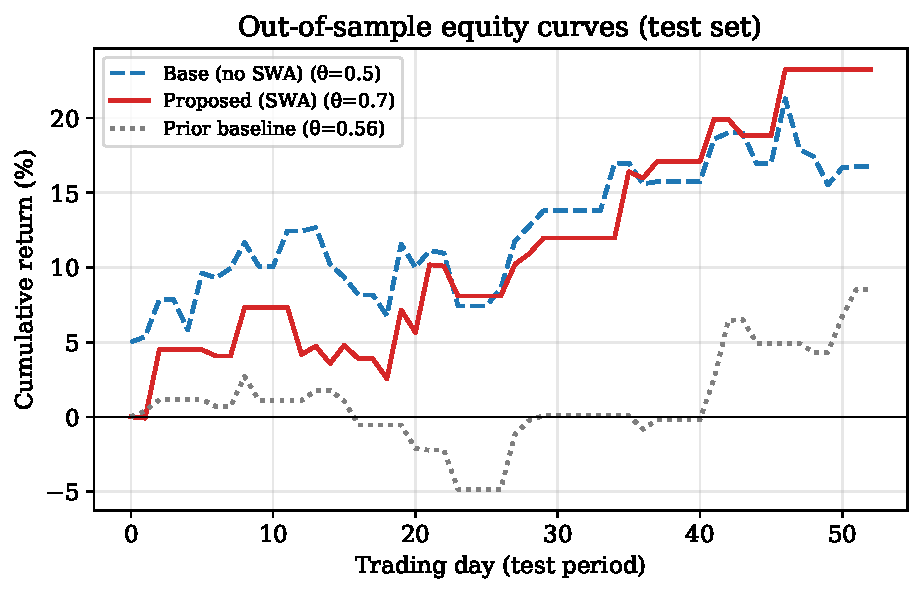
\includegraphics[width=0.85\textwidth]{fig_equity_curves.pdf}
\caption{Out-of-sample cumulative return over the 53-day test window for the
prior baseline, the non-averaged model and the proposed SWA model.}
\label{fig:equity}
\end{figure}

\subsection{Ablation: effect of SWA}
Table~\ref{tab:ablation} isolates SWA on the deployed (validation-selected) seed.
For this checkpoint, averaging the final-phase weights improves the Sharpe ratio
from $2.88$ to $4.21$ and reduces the maximum drawdown from $5.2\%$ to $4.5\%$.
We caution against over-reading this within-seed gain: as shown in
Section~\ref{sec:seed}, SWA helped three of five seeds and hurt two, and did not
improve the across-seed mean. The honest reading is therefore that SWA yielded
the single best validation-selected model in our runs, not that it uniformly
improves generalization on this corpus. We also note that the SWA model attains
a lower macro-F1 ($0.27$ vs.\ $0.40$): at the higher tuned threshold it trades
sparsely and selectively, raising risk-adjusted return while lowering nominal
classification agreement---a reminder that accuracy and risk-adjusted profit are
distinct objectives.

\begin{table}[t]
\centering
\caption{SWA ablation on the deployed (validation-selected) seed, test set.
Within-seed deltas; see Section~\ref{sec:seed} for the across-seed picture.}
\label{tab:ablation}
\begin{tabular}{lccccc}
\toprule
Configuration & SR & CR & MD & macro-F1 & accuracy \\
\midrule
Base (no SWA) & $2.88$ & $+0.168$ & $0.052$ & $0.395$ & $0.438$ \\
+ SWA         & $\mathbf{4.21}$ & $\mathbf{+0.233}$ & $\mathbf{0.045}$ & $0.269$ & $0.363$ \\
$\Delta$ relative & $+46\%$ & $+39\%$ & $-15\%$ & $-32\%$ & $-17\%$ \\
\bottomrule
\end{tabular}
\end{table}

\subsection{Seed robustness}
\label{sec:seed}
Because the validation set spans few unique dates, single-seed test estimates
carry substantial variance. Table~\ref{tab:seed} reports the distribution over
five seeds of the deployed configuration; in every case the operating
checkpoint is chosen by the validation criterion before being measured on test.
The variance is large for both variants (test-SR standard deviation $\approx
1.8$--$2.0$), and three observations follow. First, the headline figure
(SR~$4.21$) corresponds to the seed with the highest validation Sharpe ($5.54$),
i.e.\ it is the \emph{validation-selected operating point}, not an expected
value. Second, SWA improved three of the five seeds but degraded the other two,
so it does \emph{not} raise the across-seed mean in this regime; its concrete
benefit here is to produce the single best validation-selected checkpoint.
Third, the wide spread is itself the central empirical message: with $53$ test
dates, point estimates of risk-adjusted return are statistically fragile and
must be read as such.

\begin{table}[t]
\centering
\caption{Per-seed validation and test Sharpe for the deployed configuration; the
operating threshold $\theta$ is tuned on validation per seed. The deployed model
is the SWA checkpoint of the validation-selected seed (seed~2, highest SWA
validation Sharpe, $5.54$); the \emph{base} row reports the same seed's
non-averaged checkpoint for a controlled within-seed ablation (both shown in
bold). The last two columns give the across-seed mean and sample standard
deviation of the test Sharpe.}
\label{tab:seed}
\setlength{\tabcolsep}{4.5pt}
\begin{tabular}{llccccccc}
\toprule
Variant & metric & s0 & s1 & s2 & s3 & s4 & mean & std \\
\midrule
\multirow{2}{*}{Base}
 & val SR  & $6.08$ & $5.53$ & $\mathbf{3.57}$ & $6.27$ & $5.57$ & --- & --- \\
 & test SR & $-0.19$ & $3.28$ & $\mathbf{2.88}$ & $2.76$ & $-0.22$ & $+1.70$ & $1.75$ \\
\midrule
\multirow{2}{*}{SWA}
 & val SR  & $2.69$ & $4.05$ & $\mathbf{5.54}$ & $4.31$ & $2.44$ & --- & --- \\
 & test SR & $0.08$ & $-0.17$ & $\mathbf{4.21}$ & $-0.49$ & $0.09$ & $+0.75$ & $1.95$ \\
\bottomrule
\end{tabular}
\end{table}

\subsection{Per-asset analysis}
Figure~\ref{fig:perasset} decomposes the SWA model by instrument. The strategy
is profitable on seven of twelve assets (notably TSLA, ETH and MRNA, with
per-asset Sharpe above $2.5$) and loses on five (ADBE and BMRN being the worst).
This heterogeneity indicates that a single shared model does not transfer
uniformly across instruments and motivates instrument-aware calibration as
future work.

\begin{figure}[t]
\centering
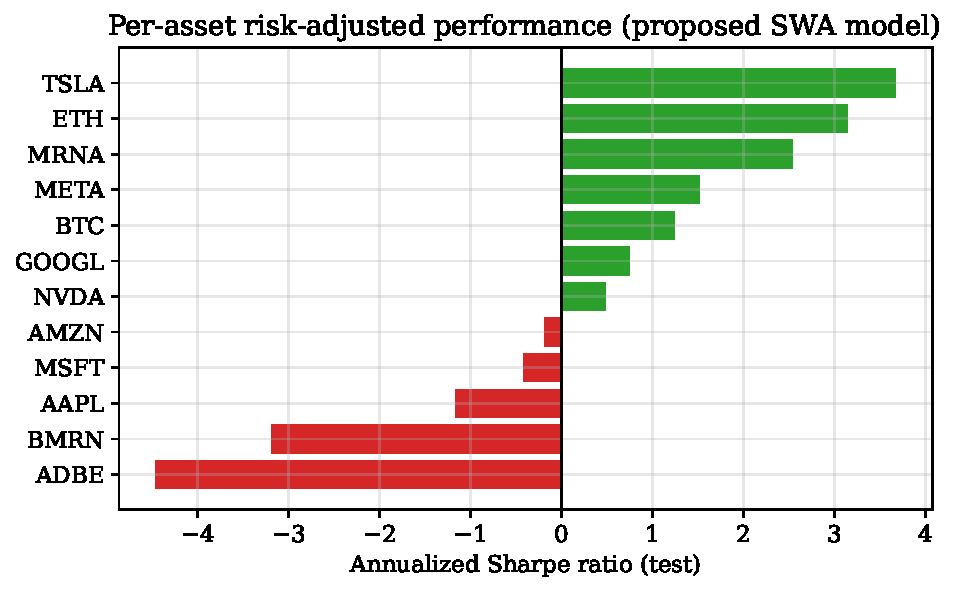
\includegraphics[width=0.82\textwidth]{fig_per_asset_sharpe.pdf}
\caption{Per-asset annualized Sharpe ratio on the test set for the proposed SWA
model. Green: profitable; red: unprofitable.}
\label{fig:perasset}
\end{figure}

\subsection{Negative result: ensembling}
Contrary to the usual variance-reduction expectation, both a five-seed ensemble
and a top-$k$ configuration ensemble \emph{degraded} out-of-sample performance.
The five-seed probability-averaging ensemble of the deployed configuration
reached a test Sharpe of $+0.81$ (CR $+2.9\%$), far below the
validation-selected single model and below the base across-seed mean. Averaging
weights systematically wrong members equally with good ones; given the large
seed variance documented in Section~\ref{sec:seed}, a subset of members
collapses toward the majority \textsc{hold} prior and the average inherits that
collapse. We conclude that, with a validation set of low temporal cardinality,
member filtering is a prerequisite for ensembling, and we adopt a
single-model-with-SWA strategy instead.

\subsection{Training dynamics and confusion structure}
Figure~\ref{fig:training} shows that the training loss decreases smoothly while
the validation Sharpe (at fixed threshold) is highly volatile---direct evidence
for the small-sample argument motivating our threshold policy. Validation
macro-F1 is comparatively stable, which is why it anchors the selection score.
Figure~\ref{fig:confusion} shows the test confusion matrix of the SWA model;
the high tuned threshold concentrates predictions on \textsc{hold}, with the
active classes used selectively.

\begin{figure}[t]
\centering
\begin{minipage}{0.56\textwidth}
\centering
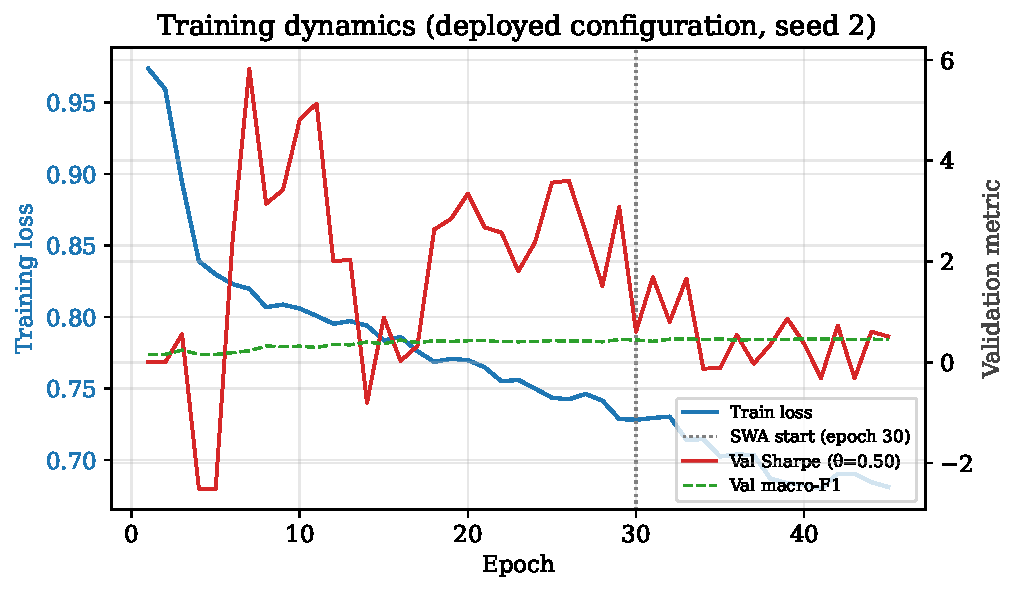
\includegraphics[width=\textwidth]{fig_training_curves.pdf}
\caption{Training loss (left axis) and validation metrics (right axis). The
dotted line marks the SWA start epoch.}
\label{fig:training}
\end{minipage}\hfill
\begin{minipage}{0.40\textwidth}
\centering
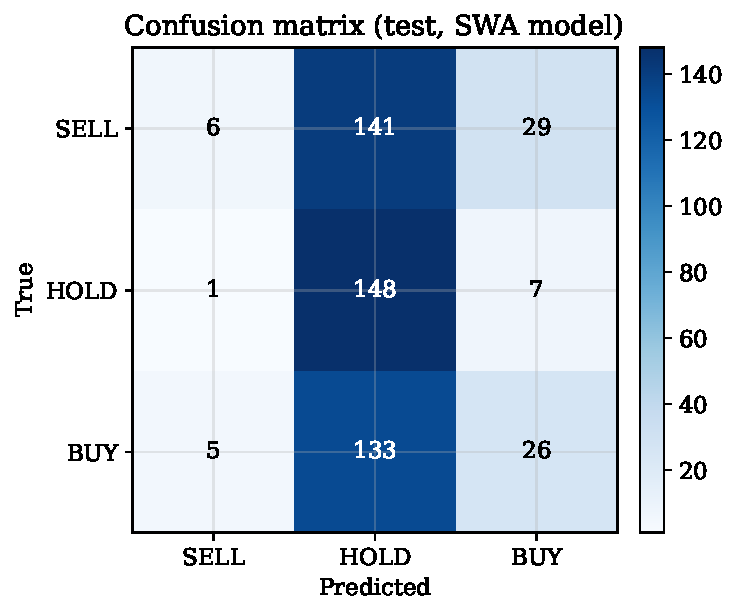
\includegraphics[width=\textwidth]{fig_confusion_matrix.pdf}
\caption{Test confusion matrix (SWA model).}
\label{fig:confusion}
\end{minipage}
\end{figure}

% ---------------------------------------------------------------------------
\section{Discussion and Limitations}
% ---------------------------------------------------------------------------
The improvements stem from pipeline-level engineering---volatility-adaptive
labelling, the separation of model and decision optimization, and SWA---rather
than from radical architectural novelty, suggesting that in multimodal problems
with limited data the binding constraint is often the experimental protocol
rather than model capacity.

Several limitations must be stated explicitly. \emph{(i) Short evaluation
horizon.} The test set spans only $53$ unique trading dates ($\approx$2.5
months); an annualized Sharpe obtained by scaling a short-window mean-to-standard
deviation ratio by $\sqrt{252}$ has wide confidence intervals, and we did not
compute bootstrap intervals. The headline figure should therefore be read as
indicative, not definitive. \emph{(ii) Small validation set.} With $40$ unique
dates, the single threshold tuned on validation is itself a high-variance
estimate. \emph{(iii) Seed sensitivity.} Performance varies strongly across seeds
(test-SR standard deviation $\approx 1.8$--$2.0$); the deployed checkpoint was
chosen by validation score, but the across-seed mean is far below the deployed
value and SWA does not improve that mean (Table~\ref{tab:seed}). The
contribution of this paper is therefore better stated as a study of protocol
under data scarcity than as a claim of a robustly superior model. \emph{(iv) No transaction
costs or slippage} are modelled, and the equal-weight active-position portfolio
is a simplification. \emph{(v) Data-source provenance.} The competition-venue
metadata could not be independently verified and is reported as provided.

% ---------------------------------------------------------------------------
\section{Conclusion}
% ---------------------------------------------------------------------------
We presented a gated multimodal architecture that fuses price series, FinBERT
news embeddings and corporate filings through availability-masked gating, and we
validated it on the FinMMEval Task~3 corpus. The validation-selected model,
combining per-asset adaptive labelling, decoupled threshold optimization and
Stochastic Weight Averaging, achieved a test cumulative return of $23.3\%$, a
Sharpe ratio of $4.21$ and a maximum drawdown of $4.45\%$. We reported these as
validation-selected operating points and showed, through a seed study, that the
across-seed distribution is wide and that neither SWA nor ensembling robustly
improves the mean in this short-horizon regime---results we present as a
methodological caution rather than as a universally superior model. Future work
includes bootstrap confidence intervals over a longer test horizon, filtered
ensembling, instrument-aware calibration, and parameter-efficient fine-tuning of
the text encoder.

\begin{credits}
\noindent\textbf{Acknowledgments.} The authors thank the organizers of the
FinMMEval shared task for assembling and releasing the dataset used in this work.

\noindent\textbf{Disclosure of Interests.} The authors declare no competing
interests.
\end{credits}

% ---------------------------------------------------------------------------
\begin{thebibliography}{99}

\bibitem{izmailov2018}
Izmailov, P., Podoprikhin, D., Garipov, T., Vetrov, D., Wilson, A.G.:
Averaging Weights Leads to Wider Optima and Better Generalization.
In: Proc.\ Uncertainty in Artificial Intelligence (UAI), pp.\ 876--885 (2018)

\bibitem{nie2023}
Nie, Y., Nguyen, N.H., Sinthong, P., Kalagnanam, J.:
A Time Series is Worth 64 Words: Long-term Forecasting with Transformers.
In: Int.\ Conf.\ on Learning Representations (ICLR) (2023)

\bibitem{yang2020}
Yang, Y., Uy, M.C.S., Huang, A.:
FinBERT: A Pretrained Language Model for Financial Communications.
arXiv:2006.08097 (2020)

\bibitem{araci2019}
Araci, D.:
FinBERT: Financial Sentiment Analysis with Pre-trained Language Models.
arXiv:1908.10063 (2019)

\bibitem{vaswani2017}
Vaswani, A., Shazeer, N., Parmar, N., Uszkoreit, J., Jones, L., Gomez, A.N.,
Kaiser, {\L}., Polosukhin, I.:
Attention is All You Need.
In: Advances in Neural Information Processing Systems (NeurIPS), pp.\ 5998--6008 (2017)

\bibitem{loshchilov2019}
Loshchilov, I., Hutter, F.:
Decoupled Weight Decay Regularization.
In: Int.\ Conf.\ on Learning Representations (ICLR) (2019)

\bibitem{arevalo2017}
Arevalo, J., Solorio, T., Montes-y-G{\'o}mez, M., Gonz{\'a}lez, F.A.:
Gated Multimodal Units for Information Fusion.
In: ICLR Workshop Track (2017). arXiv:1702.01992

\bibitem{baltrusaitis2019}
Baltru\v{s}aitis, T., Ahuja, C., Morency, L.-P.:
Multimodal Machine Learning: A Survey and Taxonomy.
IEEE Trans.\ Pattern Anal.\ Mach.\ Intell.\ \textbf{41}(2), 423--443 (2019)

\bibitem{ke2017}
Ke, G., Meng, Q., Finley, T., Wang, T., Chen, W., Ma, W., Ye, Q., Liu, T.-Y.:
LightGBM: A Highly Efficient Gradient Boosting Decision Tree.
In: Advances in Neural Information Processing Systems (NeurIPS), pp.\ 3146--3154 (2017)

\bibitem{ding2015}
Ding, X., Zhang, Y., Liu, T., Duan, J.:
Deep Learning for Event-Driven Stock Prediction.
In: Proc.\ Int.\ Joint Conf.\ on Artificial Intelligence (IJCAI), pp.\ 2327--2333 (2015)

\bibitem{hu2018}
Hu, Z., Liu, W., Bian, J., Liu, X., Liu, T.-Y.:
Listening to Chaotic Whispers: A Deep Learning Framework for News-oriented Stock
Trend Prediction.
In: Proc.\ ACM Int.\ Conf.\ on Web Search and Data Mining (WSDM), pp.\ 261--269 (2018)

\bibitem{sezer2020}
Sezer, O.B., Gudelek, M.U., Ozbayoglu, A.M.:
Financial Time Series Forecasting with Deep Learning: A Systematic Literature
Review: 2005--2019.
Applied Soft Computing \textbf{90}, 106181 (2020)

\bibitem{szegedy2016}
Szegedy, C., Vanhoucke, V., Ioffe, S., Shlens, J., Wojna, Z.:
Rethinking the Inception Architecture for Computer Vision.
In: Proc.\ IEEE Conf.\ on Computer Vision and Pattern Recognition (CVPR),
pp.\ 2818--2826 (2016)

\bibitem{lopezdeprado2018}
L{\'o}pez de Prado, M.:
Advances in Financial Machine Learning.
Wiley, Hoboken, NJ (2018)

\bibitem{sharpe1994}
Sharpe, W.F.:
The Sharpe Ratio.
Journal of Portfolio Management \textbf{21}(1), 49--58 (1994)

\end{thebibliography}

\end{document}
